\section{Лекция 1. Алгебра конечных регулярных выражений и конечные автоматы.}

\begin{Def}
    $\textbf{\text{Алфавит}} \sum$ - любое $\underline{\text{конечное}}$ множество.
\end{Def}

\begin{Def}
    $\textbf{\text{Слово}}$  - $\underline{\text{конечная}}$ последовательность символов из алфавита.
\end{Def}

\begin{Def}
    $\textbf{\text{Конкатенация}}$  - операция сцепки. Пусть $w, v$ - слова, где $w = aba$, а $v = bb$, тогда конкатенация этих слов: $w \circ v = ababb$
\end{Def}

\begin{Def}
    $ \sum^{*}$ - $\text{множество всех слов } \text{над алфавитом } \sum$
\end{Def}

\begin{Def}
    $\textbf{Язык } L$ - подмножество множества всех слов $\sum^{*}$.
\end{Def}

\begin{Def}
    Пусть $u = ababb$, тогда $u[i]$ - это $\textbf{i-тая буква}$ в слове $u$. $u[1] = a$, $u[i, j] = u[i]\circ u[i + + 1] \circ \dotsc \circ u[j]$, например $u[1,4] = abab$
\end{Def}

\begin{Def}
    \textbf{Длина слова } $|w|$ - количество символов в слове $w$.
\end{Def}

\begin{Def}
    $\textbf{Пустое слово } \varepsilon$ - специальное слово, для которого выполняется:
    \begin{enumerate}
        \item $\forall w \in \sum^{*} \implies w \circ \varepsilon = \varepsilon \circ w = w$
        \item $|\varepsilon| = 0$
    \end{enumerate}
\end{Def}

\begin{Def}
    Пусть $x \in \sum^{*}$, тогда $x^n = \underbrace{x \circ x  \circ \dots \circ x}_{n}$, нулевая степень: $x^0 = \varepsilon$

\end{Def}
\begin{Def}
    Слово $u$ называется \textbf{подсловом} слова $w$, если существуют такие слова $x$ и $z$, что $w = x\circ u \circ z$
\end{Def}

\begin{question}
    Сколько подслов у слова $aba$?
\end{question}

\begin{nonum}
    6 подслов: $ \varepsilon , a, b, ab, ba, aba$
\end{nonum}

\begin{Def}
    Пусть $w, u \in \sum^{*}$, тогда $|w|_{u}$ - \textbf{количество различных вхождений} слова $u$ в слово $w$ как подслова
\end{Def}
Например, пусть $w = ababa$, а $u = aba$, тогда $|w|_u = |w|_{aba} = 2$

\begin{center}
    \textit{Операции на языках}
\end{center}

\begin{enumerate}
    \item \textbf{Конкатенация}: $X \circ Y = \{ x \circ y | x \in X, y \in Y\}$
    \item \textbf{Возведение в степень:} $X^n = \underbrace{X\circ X \circ \dots \circ X}_{n}$, при $n \geqslant 1$, если же $n = 0$ и $X \neq \varnothing$, то $X^0 = \varepsilon$. Пустое множество возводить в нулевую степень \textbf{нельзя}.
    \item \textbf{Объединение:} $X|Y = X + Y = X \cup Y$
    \item \textbf{Итерация} или \textbf{звёздочка Клини}: $X^{*} = \varepsilon + X + X^2 + X^3 + \dotsc + X^n + \dotsc$
    \item $X^+ = X \circ X^*$
\end{enumerate}
P.S. Язык состоящий из одного слова отождествляется со словом, ровно как и слово состоящие из одного символа является буквой алфавита.

\begin{Def}
    \textbf{Класс регулярных языков REG}:
\end{Def}
\begin{enumerate}
    \item $\varnothing \in REG$
    \item $\forall\sigma \in \sum \implies \{\sigma\} \in  REG$
    \item $\forall X, Y \in REG: X \circ Y, X|Y, X^* \in REG$
\end{enumerate}

Регулярные языки и только они могут быть заданы при помощи регулярных выражений, например выражение $a(a|bb)$ задаёт регулярный язык $L = \{aa, abb\}$


\begin{question} Докажите, что следующие языки являются регулярными:
    \textbf{а)} язык, состоящий из одного слова; \textbf{б)} любой конечный язык; \textbf{в)} язык всех слов; \textbf{г)}язык, состоящий только из пустого слова.
\end{question}

\begin{nonum}
    Доказательство проще всего приводить, начиная самого последнего пункта. Пусть язык $L$ состоит только из пустого слова, тогда он является регулярным. Действительно рассмотрим вспомогательный язык $P = \{\varnothing\}$, он является регулярным по первому пункту определения класса REG, а значит $P^{*} = \{\varepsilon\}$ тоже является регулярным языком уже по третьему пункту того же определения. Таким образом, пункт \textbf{г)} доказан.

    Вернемся к началу и докажем пункт \textbf{а)}. Если язык состоит из одного слова, и это слово не является пустым словом, то язык регулярный, так как слово - конечная последовательность символов, то есть конечная конкатенация языков, состоящих только из одного символа (все они регулярные по второму пункту определения регулярности языков), и тогда наш начальный язык - регулярный по индукции и по третьему пункту определения регулярного языка, если же это единственное слово - пустое, то язык регулярный по пункту \textbf{г)}. Пункт \textbf{а)} доказан

    Доказательство пункта \textbf{б)} проведём по индукции по количеству слов в языке. База индукции - пустое множество. Такой язык является регулярным по первому пункту определения класса REG языков. Предположим, что язык $X$, состоящий из $k$ слов является регулярным и попробуем построить переход. Для этого рассмотрим язык $Y$, который состоит из одного слова, которого нет в $X$. $Y$ является регулярным языком по всё тому же пункту \textbf{б)}. Теперь рассмотрим новый язык $Z = X|Y$, в нём $k + 1$ слов и по третьему пункту определения регулярного языка $Z$ - принадлежит классу REG. Переход построен, и доказательство завершено.

    Теперь на основе пункта \textbf{б)} мы можем доказать и пункт \textbf{в)}. Рассмотрим в качестве языка алфавит $\sum$, каждое слово которого состоит из одного символа. Этот язык конечный в силу определения алфавита, а значит по пункту \textbf{б)} он принадлежит классу регулярных. Тогда применим к алфавиту операцию итерации (звёздочку Клини), тогда по третьему пункту определения регулярных языков язык всех слов будет являться регулярным.

\end{nonum}


\begin{question} Решив предыдущий контрольный вопросв, вы доказали, что каждое слово по отдельности - регулярный язык. Возьмём произвольный язык $L \subseteq \sum^{*}$ и представим его в виде объединения всех входящих в него слов:
    \begin{equation}
        L = \bigcup_{w \in L}{w}
    \end{equation}
    Глядя на эту формулу, некоторые студенты заключают, что раз регулярные языки замкнуты относительно объединения, то $L$ - регулярный язык. Значит, нерегулярных языков не бывает в силу произвольности L! В чём ошибка в этом рассуждений!
\end{question}
\begin{nonum}
    Проблема в предложенном решении состоит в том, что язык $L$ может оказаться бесконечным, и тогда не получится применить индукцию.
\end{nonum}

\begin{center}
    \textit{Конечные автоматы}
\end{center}

\begin{figure}[htp]
    \centering
    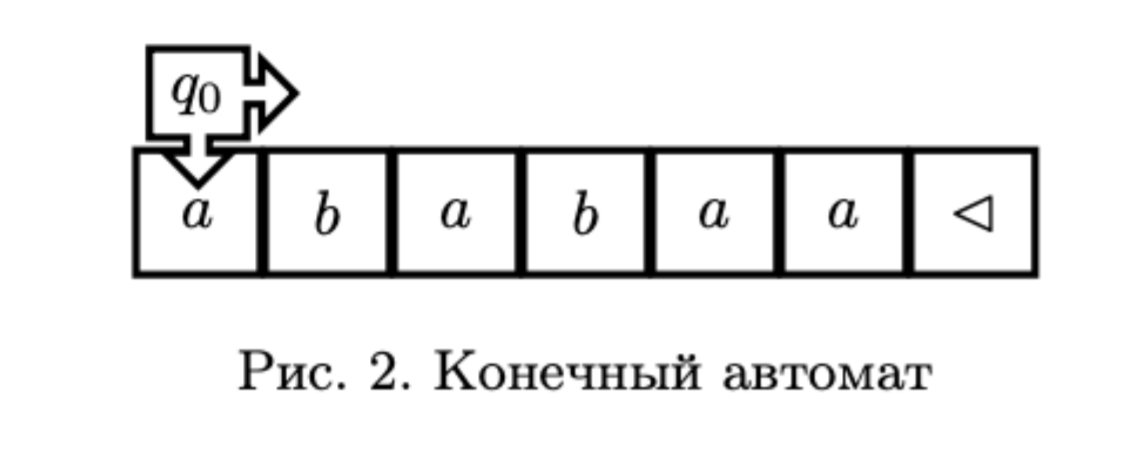
\includegraphics[width=8cm]{images/FiniteAutoma.PNG}
    \label{fig:stateMachine}
\end{figure}

\begin{Def}
    \textbf{Детерминированный конечный автомат}. Пусть:
    \begin{enumerate}
        \item $\sum$ - алфавит
        \item $Q$ - конечное множество состояний
        \item $q_0 \in Q$ - начальное состояние
        \item $F \subseteq Q$ - множество принимающих состояний
        \item $\delta$ - частично определенная функция перехода
              из множества $Q \times \sum$ в множество $Q$
    \end{enumerate}
\end{Def}